\documentclass[acmtog, nonacm]{acmart}

\begin{document}

\title{State of the ART: The Adaptive Radix Tree Index for Main-Memory Databases}

\author{Jonas Fritsch}
\affiliation{
    \institution{Technische Universtität München}
    \department{Fakultät für Informatik}}
\email{fritsch@in.tum.de}

\begin{abstract}
    With recent trends in hardware, main memory capacities have grown to an extent where most traditional DBMS 
    can fit entirely into memory. This change introduced a new shift of the performance bottleneck 
    from disk-based I/O to main memory access.
    
    While previous index structures like the B-Tree were optimized for minimizing disk access, the 
    adaptive radix tree (ART) is a trie-based index structure designed explicitly for in-memory usage. 
    It utilizes newer architecture features like SIMD and caching effectively and compresses its structure 
    dynamically, both horizontal and vertical. With these measures, ART achieves a performance that beats 
    other state-of-the-art order-preserving indexes in both insertion and single-lookup time while having also
    having a lower memory footprint.
\end{abstract}

\maketitle

\section{Introduction}
The architecture of DBMS has constantly been evolving due to advances in hardware. 
Over the last few decades, main memory capacities increased from several megabytes up to thousands 
of gigabytes, such that nowadays, databases can fit entirely into main memory. This change significantly 
impacted the general architecture of DBMS, which resulted in performance improvements 
by several factors \cite{10.1145/1376616.1376713}, \cite{7097722}.

The design of index structures used to query a set of data more efficiently was heavily influenced 
by the main performance bottleneck of disk I/O in traditional disk-based DBMS. 
Original index structures like the B-Tree designed to minimize disk accesses perform poorly 
in an in-memory environment. 
The T-Tree \cite{lehman1985study} was one of the first index structures proposed for main memory DBMS. 
However, over the last 35 years, the hardware landscape changed dramatically, causing T-Trees 
and all other index structures not explicitly designed with caching effects in mind to be rendered 
inefficient \cite{rao1998cache}. Further focus on developing cache-sensitive index structures resulted in many 
different search tree variants.

Cache-sensitive search trees (CSS-Trees) \cite{rao1998cache}, while utilizing cache lines efficiently, 
introduce a significant overhead for updates as the tree is compactly stored in an array. 
Similarly, the more recent k-ary search tree \cite{10.1145/1565694.1565705} and the Fast Architecture 
Sensitive Tree (FAST) \cite{10.1145/1807167.1807206} both utilize Single Instruction Multiple Data (SIMD) 
instructions for data-level parallelism (DLP) to increase performance. However, as static data 
structures, they do not support incremental updates. A way to circumvent this limitation is to 
use a delta mechanism where another data structure stores differences and is periodically merged 
into the static structure. This comes at an additional performance cost. The cache-conscious 
B\textsuperscript{+}-Tree (CSB\textsuperscript{+}) \cite{10.1145/342009.335449} introduced as a variant of 
B\textsuperscript{+}-Trees improves cache utilization by reducing the need to store all different 
child pointers in each node.

Hash-Tables have been a popular indexing choice for main memory databases as they provide 
optimal $O(1)$ - as opposed to $O(\log n)$ for search trees - single-lookup and update 
time on average. Many different hashing schemes and hash functions have been developed 
over time, but hash-tables generally do not support any range-based queries due to the nature 
of hash functions. Additionally, hash-tables can require complete re-hashing with $O(n)$ complexity 
upon reaching its load balance.

Another possible data structure used for indexing is a trie, also called prefix tree. Tries are search trees 
with the difference that keys are inserted in pieces (partial keys). This means that two keys sharing a common
prefix will have the same path from the root until their next partial key differs. A radix tree, sometimes also called Patricia-Trie, is a variant of
a trie that further compactifies its structure by compressing nodes for partial keys that only have one child, as 
shown in Figure \ref{fig:trie}. With radix trees, some form of leaf nodes holding the compressed rest key is required 
to restore full keys.

\begin{figure}
    \centering
    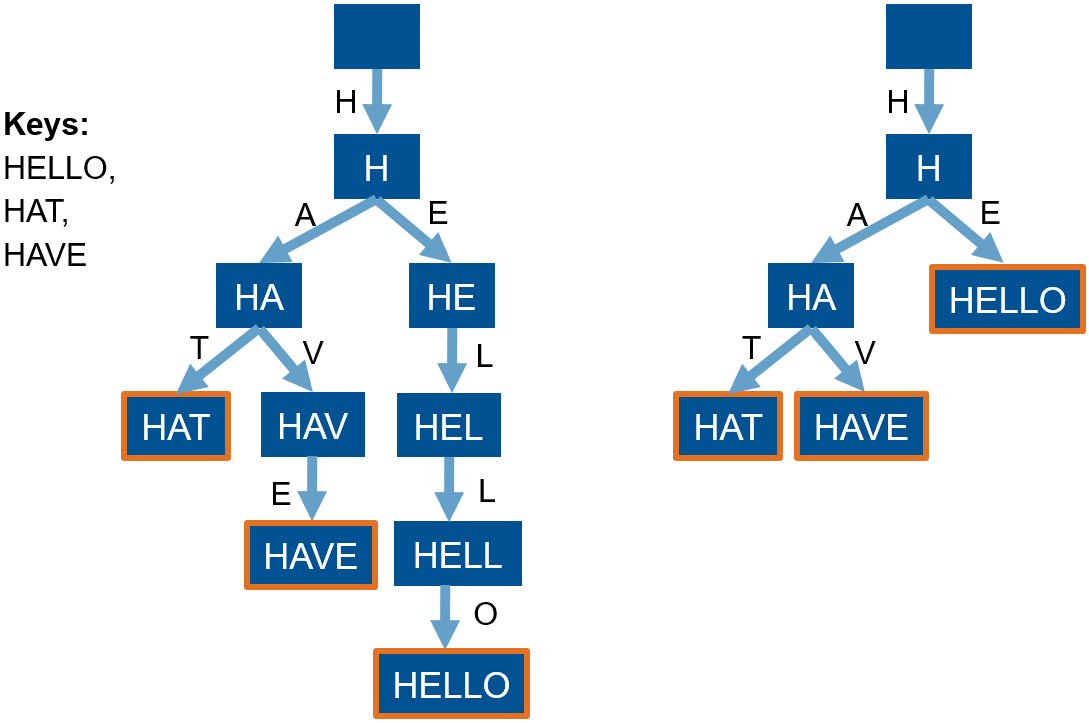
\includegraphics[width=0.5\textwidth]{images/01-trie-radix-tree-example.PNG}
    \caption{A trie with span 8 (1 byte per character) storing the keys HELLO, HAT, and HAVE on the left and its radix tree variant on the right. Nodes marking the end of a word are outlined.}
    \label{fig:trie}
\end{figure}

Tries have the following interesting properties:
\begin{itemize}
    \item Tree height and complexity do not depend on the number of keys $n$ stored but rather
    the key length $k$. As we will see later in Section 4, this means that its performance is mainly impacted not by
    the amount of keys present as in other search trees but by the skewness of these keys.
    \item Tries require no rebalancing.
    \item All insertion orders result in the same tree.
    \item Keys are stored in lexicographic order.
    \item Keys are stored implicitly along paths. (This is not directly true for radix trees and can differ with implementations.)
\end{itemize}

The span of a trie is the number of bits making one partial key. The fanout of a node is the number of children 
a node can have maximum. The most efficient implementation for a trie of span $s$ is to have a fanout of $2^s$ on 
each node. This means that when storing the children in a pointer array of size $2^s$, the partial key can be used 
directly as index into this array to find the next child without having to make any comparisons.
With this, the height of a given trie storing keys of $k$ bits is bound by $\lceil k/s\rceil$, and increasing 
the span results in a lower trie height which is desirable as the height dictates the time complexity of almost 
all operations.

On the other hand, increasing the span results in an exponentially higher fanout, thus requiring more space as even 
if few children exist, the array will be filled with null pointers wasting memory. 
For this reason, having a very high span is generally impractical. The Generalized Prefix Tree (GPT) \cite{mci/Boehm2011} 
has a span of 4, and the radix tree implementation used in the Linux kernel uses 6 bits \cite{corbet2006lrt}. 
The Adaptive Radix Tree (ART) \cite{6544812}, as depicted in Figure \ref{fig:trie-mem}, while using a span of 8, manages to have both 
fairly low memory consumption as well as a small tree height.

\begin{figure}
    \centering
    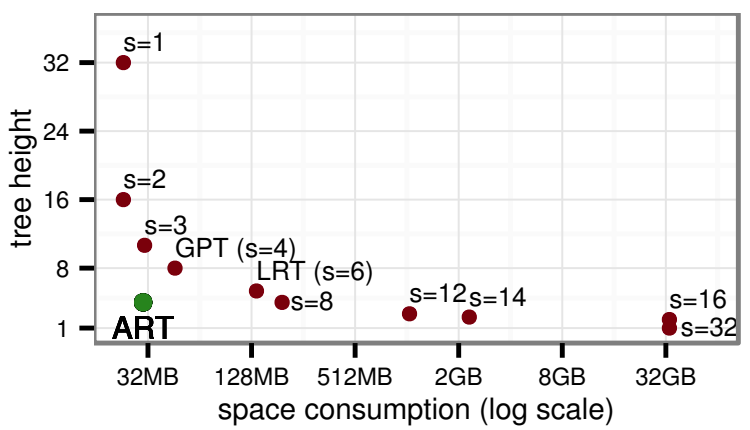
\includegraphics[width=0.4\textwidth]{images/02-trie-memory-consumption.png}
    \caption{Comparison of tree height versus space consumption for different radix tree spans $s$ when storing 1M uniformly distributed 32 bit integers with 8 byte pointers.
    Source: \cite{6544812}}
    \label{fig:trie-mem}
\end{figure}

The key idea in lowering memory consumption while maintaining a high span for tries is to adaptively use nodes 
with different fanouts based on the number of actual children. One of the first data structures to utilize such 
adaptive nodes was the Judy Array \cite{baskins2004judy} which was invented by Doug Baskins and developed at 
Hewlett-Packard research labs as a general associative array. However, due to its patent and overall complexity, 
it has not yet been researched as much. Also, its original, almost two-decade-old design has flaws like assuming 
16 byte cache-line sizes or not utilizing SIMD.

The rest of this paper is organized as follows. We first introduce the Adaptive Radix Tree as an index structure 
and explain its key design features. In Section 3, we show how to convert different key types to binary-comparable keys to 
index in ART. Section 4 evaluates ART by comparing its performance and memory consumption first in 
micro-benchmarks and then the TPC-C benchmark. Section 5 discusses related work and research done since the 
original proposition of ART back in 2013. The final part draws a conclusion and discusses future work.

\section{The Adaptive Radix Tree}
The Adaptive Radix Tree (ART) was first proposed by Leis et al. \cite{6544812} as a performant, order-preserving 
in-memory index structure. As a radix tree using multiple different node types with different fanouts, it applies 
horizontal compression to drastically lower memory consumption and vertical compression to reduce the overall tree 
height and further memory usage while improving performance.

\subsection{Horizontal Compression (Adaptive Nodes)}
Similar to Judy Arrays, ART uses a number of different node types, each with a different fanout but the same span 
of 8, to adaptively change between them based on the actual number of child nodes. This way, less space is wasted 
storing null pointers. Additionally, storing the children in sorted order allows for range scans along nodes. ART 
uses four different node types illustrated in Figure \ref{fig:nodes} and named after the maximum number of children 
they can store. For better cache line utilization during searches ART stores partial keys and child pointers in two 
seperate arrays as opposed to storing key-pointer pairs in one single array:

\begin{figure}
    \centering
    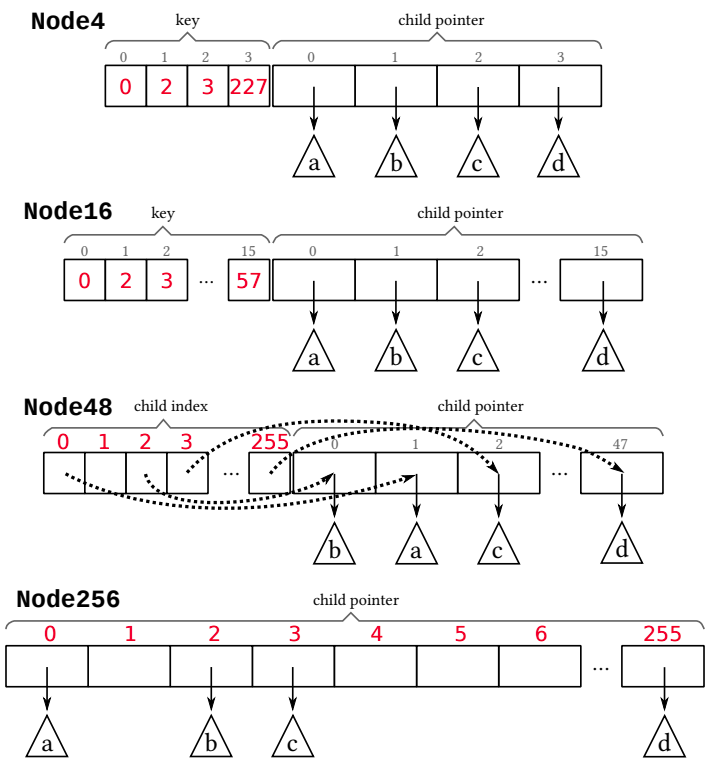
\includegraphics[width=0.5\textwidth]{images/03-art-node-types.png}
    \caption{Different node structures used by ART. For each node, the partial keys 0, 2, 3, and 255 are mapped to the subtrees a, b, c, and d, respectively.
    Source: \cite{6544812}}
    \label{fig:trie-mem}
\end{figure}

\textbf{Node4:} Stores up to 4 children by maintaining a sorted array of size 4 of partial keys where the searched index 
in the key array is directly used as index into the child pointer array.

\textbf{Node16:} This node stores up to 16 children in the same way as Node4. Searching for a key can be done 
efficiently using SIMD instructions.

\textbf{Node48:} As the number of partial keys to differentiate increases, searches become more expensive, even in 
sorted order. Therefore Node48 uses a full 256-sized byte array to hold all possible partial keys. However, as this 
node only stores up to 48 children, our child pointer array is only of size 48. ART thus stores the index into the 
child pointer array as value in the key array, which is indexed directly using the partial key.

\textbf{Node256:} Finally, the largest node stores children in the classical trie approach with a child pointer 
array of size 256 so that, similarly to Node48, the partial key is used directly as index.

Additionally, all nodes have a header of constant size storing the node type, the number of non-null children, 
and a prefix variable containing information about the compressed path (see Section 2.2).

\subsection{Vertical Compression}
As a radix tree, ART implements two techniques often used in tree-like structures: lazy expansion and path compression. 
Thus ART compresses node chains where each node only has a single child, further reducing tree height and space 
consumption while improving performance.

\textbf{Lazy Expansion:} 
Lazy expansion refers to the standard radix tree approach introduced by Morrison \cite{10.1145/321479.321481} to 
expand nodes lazily upon insertion, meaning that
nodes are only created as long as they are needed to distinguish between at least two different keys. This can be seen
again in Figure \ref{fig:art-vertical-compression} where the key FOO is lazy expanded, meaning the path for storing the
two Os is omitted. Since the path to a leaf may be compressed, this requires the full key to be stored alongside 
its value or be retrievable based on it. The latter is most often the case in database indexes, where the value 
is used as a reference to a data tuple containing the key.

\begin{figure}
    \centering
    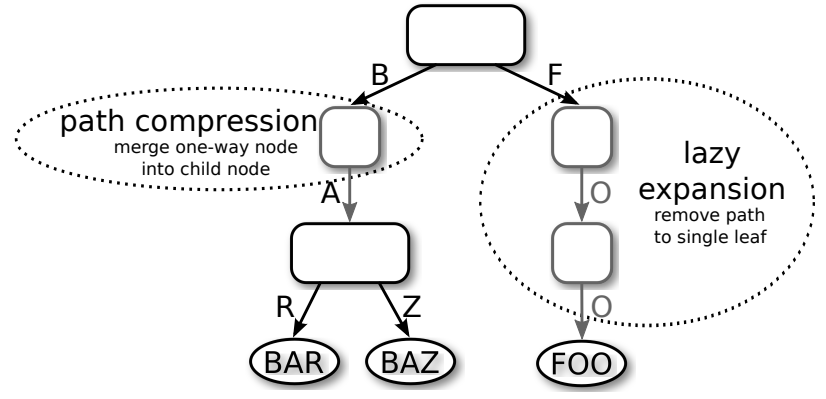
\includegraphics[width=0.45\textwidth]{images/04-art-vertical-compression.PNG}
    \caption{Lazy expansion and path compression in effect
    Source: \cite{6544812}}
    \label{fig:art-vertical-compression}
\end{figure}

\textbf{Path Compression:}

\subsection{Storing Values}

\subsection{Algorithms}

\subsection{Space Consumption}
As briefly mention in Section 1
In the original ART paper \cite{6544812} the authors proofed that on average a

\section{Constructing Binary-Comparable Keys}
Lorem ipsum.

\section{Evaluation}
Lorem ipsum.

\section{Related Work}
Lorem ipsum.

\section{Conclusion and Future Work}
Lorem ipsum.

\bibliographystyle{ACM-Reference-Format.bst}
\bibliography{refs}

\end{document}
\endinput